\chapter{Implementación}

\section{Datos}
Los datos utilizados en este trabajo han sido recopilados mediante técnicas de web scraping desde la página oficial de Sofascore \cite{Sofascore}. Para acceder a las estadísticas de un partido en dicha plataforma, basta con dirigirse a la sección ‘Estadísticas del jugador’, donde se despliega la información de todos los jugadores que participaron en el encuentro. Los mapas de calor, por su parte, se obtienen mediante una API que dispone de una función específica para tal fin.

Para incorporar los datos de un partido en la base de datos, es necesario proporcionar el nombre del jugador, el equipo, el rival correspondiente y la URL del partido; el sistema se encarga automáticamente de almacenar la información pertinente.

Dado que el código supera las cien líneas y está mayormente dedicado a ajustes relacionados con el proceso de scraping, se ha decidido no incluirlo íntegramente en este documento. No obstante, puede consultarse directamente en el repositorio disponible en GitHub.

\subsection{Mapas de calor}
Las estadísticas de los jugadores se almacenan como valores enteros o flotantes, reflejando directamente el valor cuantitativo de cada estadística (por ejemplo, 7 pases clave). Sin embargo, los mapas de calor se gestionan de manera distinta, ya que en ellos se registra una lista de pares de enteros que representan las coordenadas x e y correspondientes a las posiciones en el terreno de juego.

Para la representación gráfica del campo de fútbol se han utilizado las librerías matplotlib y mplsoccer, siendo esta última la encargada de dibujar el terreno de juego. A continuación, se muestra el código empleado para generar un campo vacío:


\begin{lstlisting}[language=Python, caption={Representación campo vacío}, label={lst:codigo-python}]
import matplotlib.pyplot as plt
from mplsoccer import Pitch

fig, ax = plt.subplots(figsize=(16, 9))
pitch = Pitch(pitch_type='opta')
pitch.draw(ax=ax)
plt.show()
\end{lstlisting}

La representación del campo vacío quedaría:

\begin{figure}[H]
    \centering
    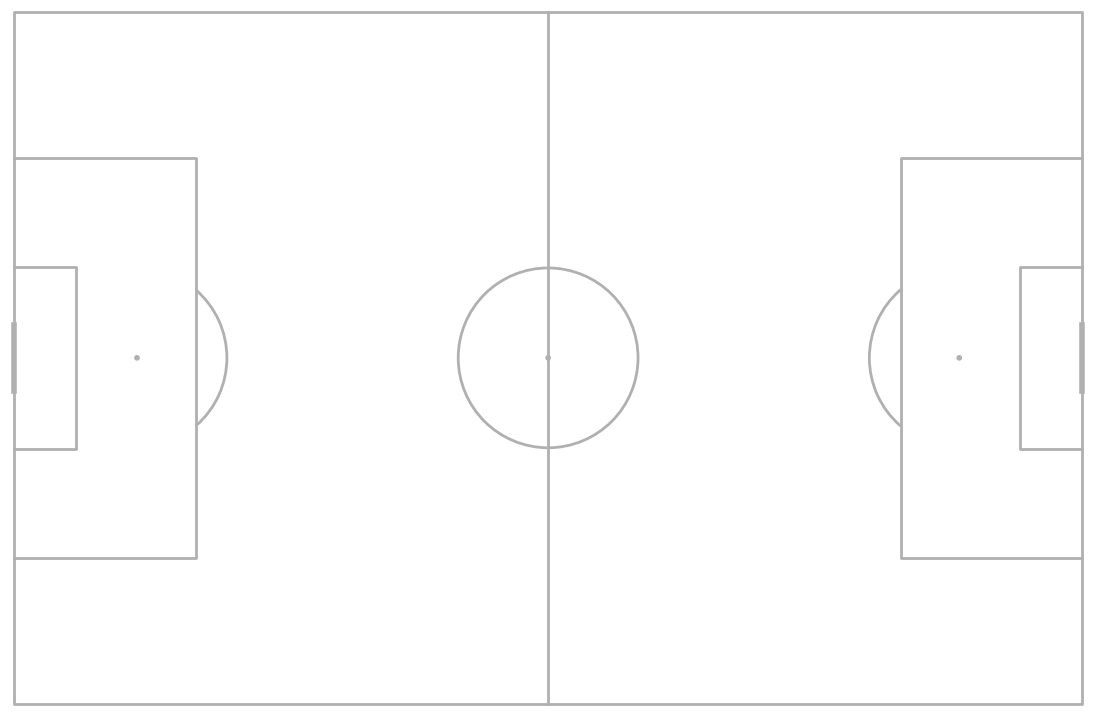
\includegraphics[width=0.7\textwidth]{plantilla-TFG-ETSIIT/doc/imagenes/Campo_vacio.png}
    \caption{Reprentación campo de fútbol}
    \label{fig:etiqueta-imagen}
\end{figure}

Es importante destacar que el punto (0, 0) corresponde a la esquina inferior izquierda del campo, mientras que el (99,99) se sitúa en la esquina superior derecha. Por ello, los mapas siempre se visualizarán de izquierda a derecha. Incluso cuando el jugador actúe como visitante, sus datos se ajustarán para mantener esta orientación constante, evitando así posibles confusiones.

Para representar el mapa de calor de un jugador específico, basta con extraer sus datos de la base de datos y graficarlos de manera similar a como se hizo anteriormente, rellenando el campo con las coordenadas correspondientes. A continuación, se presenta el código utilizado para ello:

\begin{lstlisting}[language=Python, caption={Mapa de calor de un futbolista}, label={lst:codigo-python}]

from pymongo import MongoClient
import pandas as pd
import matplotlib.pyplot as plt
from mplsoccer import Pitch
import warnings
from matplotlib.colors import LinearSegmentedColormap

warnings.filterwarnings("ignore")

# Conexion a mongoDB
cliente = MongoClient("mongodb://localhost:27017")
db = cliente["TFG"]
coleccion_jugadores = db["jugadores"]

# Buscar un jugador
jugador = coleccion_jugadores.find_one({"nombre": "Luis Milla", "equipo": "Getafe", "rival": "Villareal"})

# Verificar si se encontro el jugador
if jugador:

    mapa_calor_lista = jugador["mapa_calor"]
    mapa_calor_df = pd.DataFrame(mapa_calor_lista)
    colors = [(0, "white"), (0.5, "orange"), (1, "red")]
    custom_cmap = LinearSegmentedColormap.from_list("custom_cmap", colors)

    fig, ax = plt.subplots(figsize=(16, 9))

    pitch = Pitch(pitch_type='opta')
    pitch.draw(ax=ax)
    pitch.kdeplot(mapa_calor_df.x, mapa_calor_df.y, ax=ax,
                fill = True,
                levels=100,
                thresh=0.08,
                zorder=-1,
                bw_adjust=0.15,
                cmap="OrRd")

    # Anadir titulo personalizado
    nombre = jugador["nombre"]
    equipo = jugador["equipo"]
    rival = jugador["rival"]
    plt.title(f"Mapa de calor del jugador \"{nombre}\" del equipo \"{equipo}\", rival \"{rival}\"", fontsize=18)

    plt.show() 

else:
    print("Jugador no encontrado.")

\end{lstlisting}

Los ajustes en los valores utilizados para la representación del mapa de calor se han realizado manualmente, seleccionando aquellos que se consideraron más adecuados para una visualización clara y efectiva. A continuación, se ilustrará este proceso mediante ejemplos concretos de algunos jugadores.

El jugador Luis Milla, centrocampista del Getafe, presenta el siguiente mapa de calor correspondiente al partido disputado contra el Villarreal en la liga de la temporada 2024/2025:

\begin{figure}[H]
    \centering
    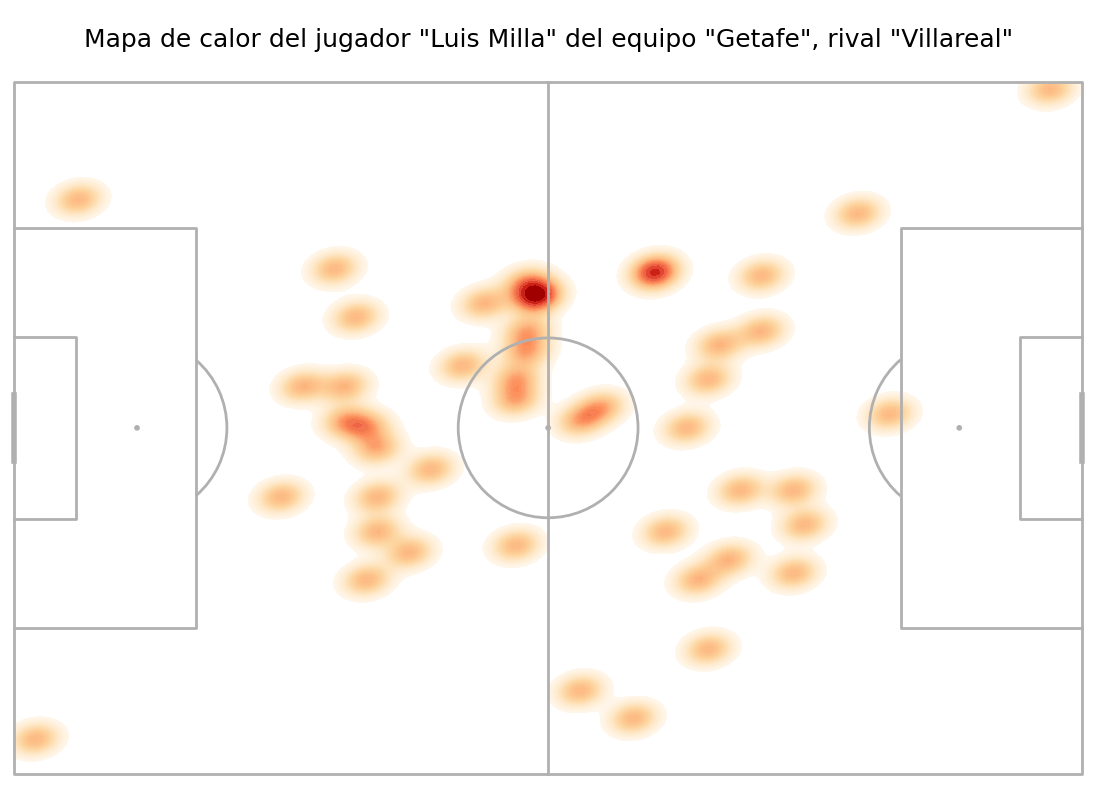
\includegraphics[width=0.7\textwidth]{plantilla-TFG-ETSIIT/doc/imagenes/Mapa_MC.png}
    \caption{Ejemplo representación de MC}
    \label{fig:etiqueta-imagen}
\end{figure}

Vamos a ver más ejemplos de otras posiciones distintas. El de un lateral derecho se vería algo así:

\begin{figure}[H]
    \centering
    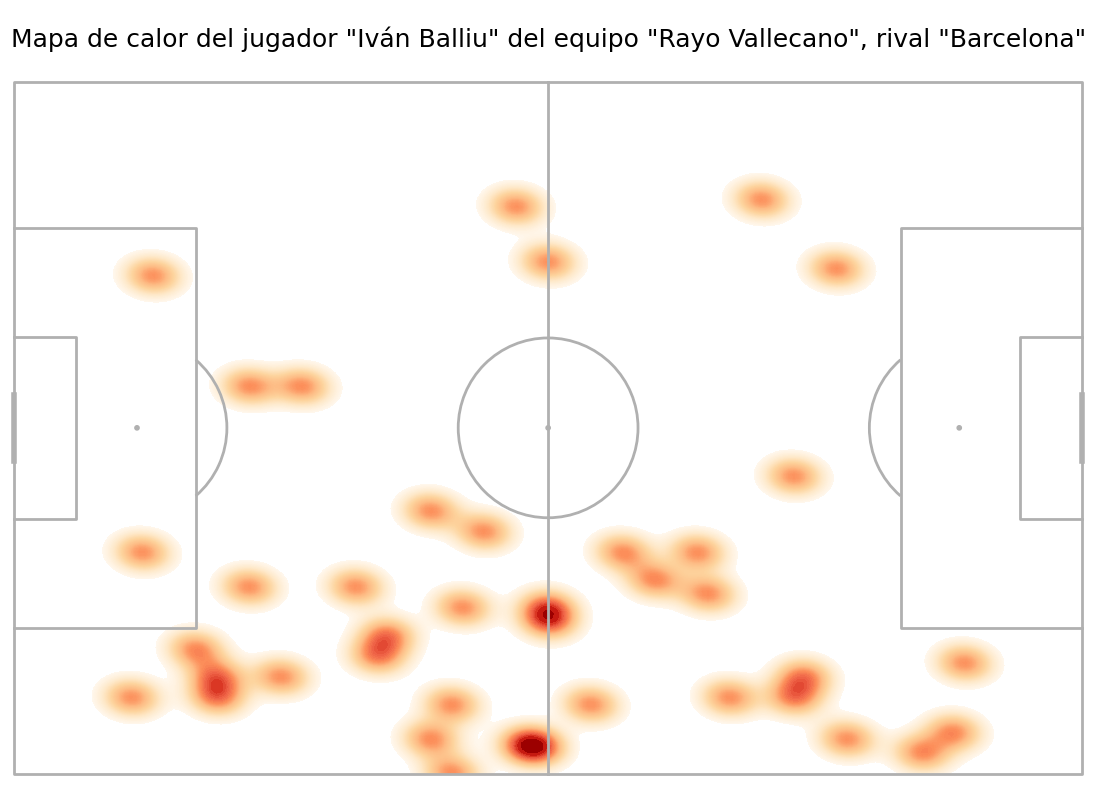
\includegraphics[width=0.7\textwidth]{plantilla-TFG-ETSIIT/doc/imagenes/Mapa_LD.png}
    \caption{Ejemplo representación de LD}
    \label{fig:etiqueta-imagen}
\end{figure}

Como se puede observar, al tratarse de un lateral derecho, su presencia predomina en la parte inferior del campo, teniendo en cuenta que la visualización del mapa se realiza de izquierda a derecha y de abajo hacia arriba.

Un ejemplo de un delantero extremo izquierdo se vería algo así:

\begin{figure}[H]
    \centering
    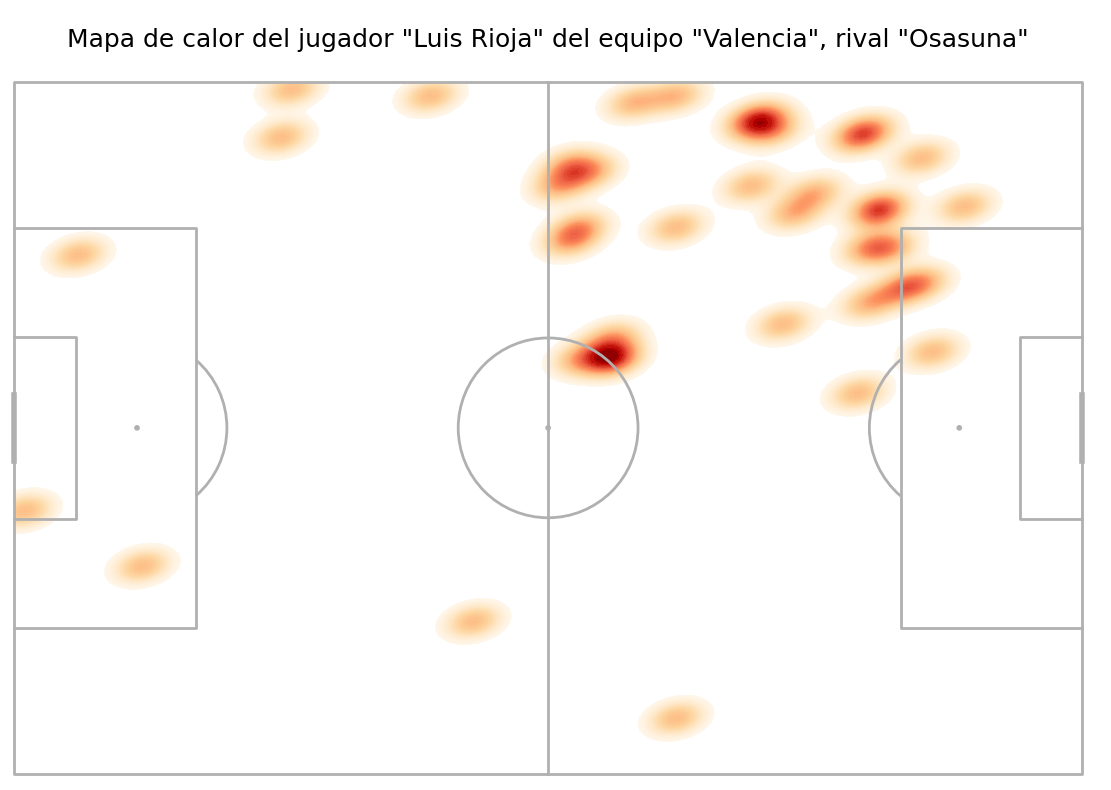
\includegraphics[width=0.7\textwidth]{plantilla-TFG-ETSIIT/doc/imagenes/Mapa_EI.png}
    \caption{Ejemplo representación de EI}
    \label{fig:etiqueta-imagen}
\end{figure}

Como se ve en la imagen, predomina principalmente la zona de arriba a la derecha, que es la que pertenece al extremo izquierdo.

Por último, vamos a ver el mapa de calor de un portero, al que rara vez vamos a ver fuera del área.

\begin{figure}[H]
    \centering
    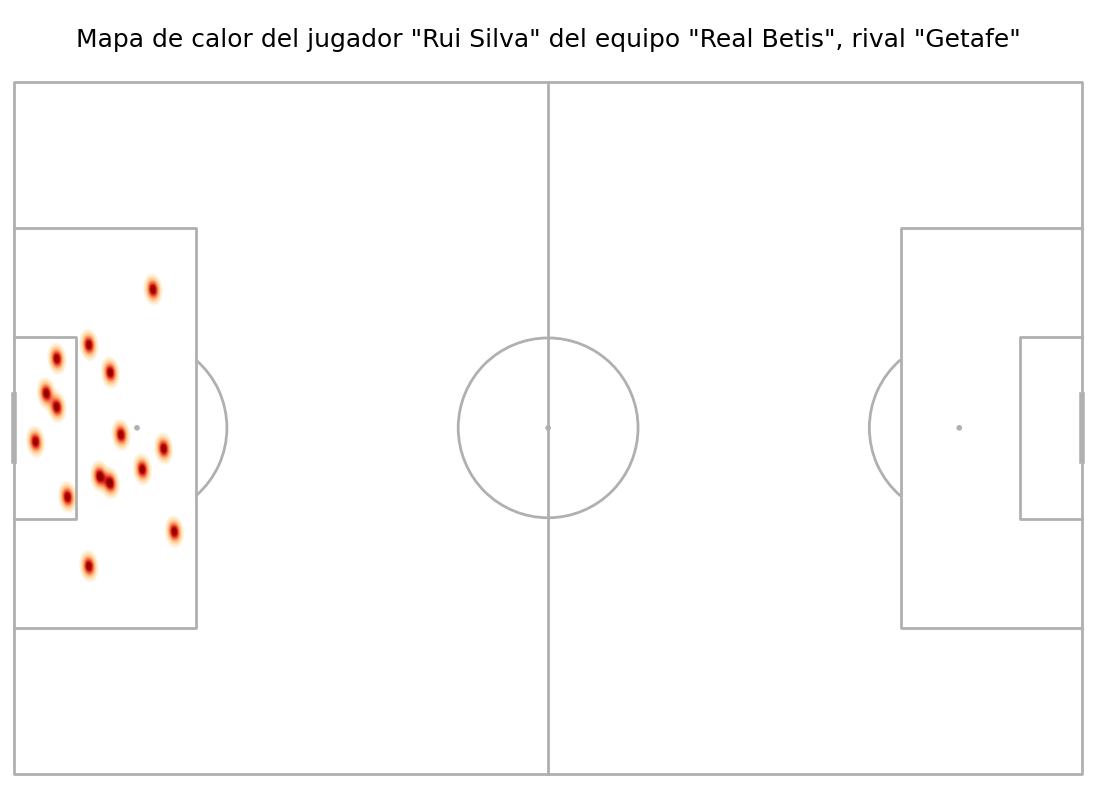
\includegraphics[width=0.7\textwidth]{plantilla-TFG-ETSIIT/doc/imagenes/Mapa_POR.png}
    \caption{Ejemplo representación de POR}
    \label{fig:etiqueta-imagen}
\end{figure}

Es importante destacar que los mapas de calor pueden presentar cierta aleatoriedad. Aunque los jugadores tienden a respetar sus posiciones habituales, en el transcurso de un partido pueden producirse situaciones inesperadas que los lleven a intervenir en otras zonas del campo, si bien estos casos son excepcionales. Por ejemplo, en el caso del extremo izquierdo, se observa que tocó el balón tres veces en su propia área, lo cual no es habitual y podría deberse a acciones defensivas en jugadas a balón parado. De manera similar, en el caso de Luis Milla, centrocampista, se aprecia que tocó el balón en las dos esquinas del campo, lo que sugiere que participó en la ejecución de saques de esquina.

\section{Algoritmo sin pesos}

Una vez obtenidos los datos de los jugadores almacenados en la base de datos, se procederá a explicar la implementación del algoritmo sin división por zonas, es decir, considerando únicamente las estadísticas individuales de los futbolistas sin segmentar el campo. No se han incluido todas las funciones debido a su extensión, pero sí se presenta la función principal del programa, que es la siguiente:

\begin{lstlisting}[language=Python, caption={Algoritmo sin zonas}, label={lst:codigo-python}]
if not JUGADORES_CACHE:
    inicializar_cache_jugadores()
#Bucle que recorre todos los partidos
for partido in coleccion_partidos.find():
    # Obtener jugadores
    jugadores1 = [jug for jug in JUGADORES_CACHE.values() if jug["equipo"] == partido["Local"] and jug["rival"] == partido["Visitante"] and jug["temporada"] == partido["Temporada"]]
    jugadores2 = [jug for jug in JUGADORES_CACHE.values() if jug["equipo"] == partido["Visitante"] and jug["rival"] == partido["Local"] and jug["temporada"] == partido["Temporada"]]
    
    maximos = calcularMaximos(jugadores1, jugadores2)

    suma_total_ofensiva_e1 = 0
    suma_total_defensiva_e1 = 0
    suma_total_ofensiva_e2 = 0
    suma_total_defensiva_e2 = 0

    for j in jugadores1:
        estadisticas_ofensivas = getEstadisticasOfensivas(j["_id"], maximos)
        estadisticas_defensivas = getEstadisticasDefensivas(j["_id"], maximos)
        suma_total_ofensiva_e1 += estadisticas_ofensivas
        suma_total_defensiva_e1 += estadisticas_defensivas
    for j in jugadores2:
        estadisticas_ofensivas = getEstadisticasOfensivas(j["_id"], maximos)
        estadisticas_defensivas = getEstadisticasDefensivas(j["_id"], maximos)
        suma_total_ofensiva_e2 += estadisticas_ofensivas
        suma_total_defensiva_e2 += estadisticas_defensivas
    
    total_e1 = suma_total_ofensiva_e1 - suma_total_defensiva_e2
    total_e2 = suma_total_ofensiva_e2 - suma_total_defensiva_e1

    resultado = total_e1 - total_e2

    if resultado > 2:
        resultado = "local"
    elif resultado < -2:
        resultado = "visitante"
    else:
        resultado = "empate"
\end{lstlisting}

Como se explicó anteriormente, este enfoque se basa únicamente en la sumatoria de las estadísticas normalizadas de todos los jugadores de cada equipo. El equipo que obtenga una puntuación total más alta será considerado el ganador.

En este caso, el umbral de decisión, fijado en el valor 2, se ha definido manualmente, ya que se trata de un algoritmo sencillo en el que no se ha aplicado ninguna técnica de \textit{machine learning}.

Las funciones 'getEstadisticasOfensivas' y 'getEstadisticasDefensivas' recorren los datos de cada jugador y extraen únicamente las estadísticas correspondientes, que han sido previamente normalizadas en un rango de 0 a 1. En esta escala, un valor de 1 representa la mejor ejecución de esa estadística dentro del partido, mientras que un valor de 0 indica el rendimiento más bajo registrado.
Los resultados de la ejecución de este algoritmo se pueden ver en la sección 6.1 en el siguiente capítulo.

\section{Algoritmo con pesos}
A continuación, se procede a la implementación del algoritmo descrito en el capítulo anterior. Tal como se indicó, el enfoque consiste en dividir el terreno de juego en 24 zonas, asignando a cada una un peso determinado en función de su relevancia para el análisis.

La distribución del campo en zonas se ha diseñado de forma que permita una evaluación más precisa del impacto de cada jugador en áreas específicas del terreno de juego. Esta segmentación facilita una interpretación más detallada del rendimiento colectivo e individual durante el partido.

La división utilizada es la siguiente:

\begin{figure}[H]
    \centering
    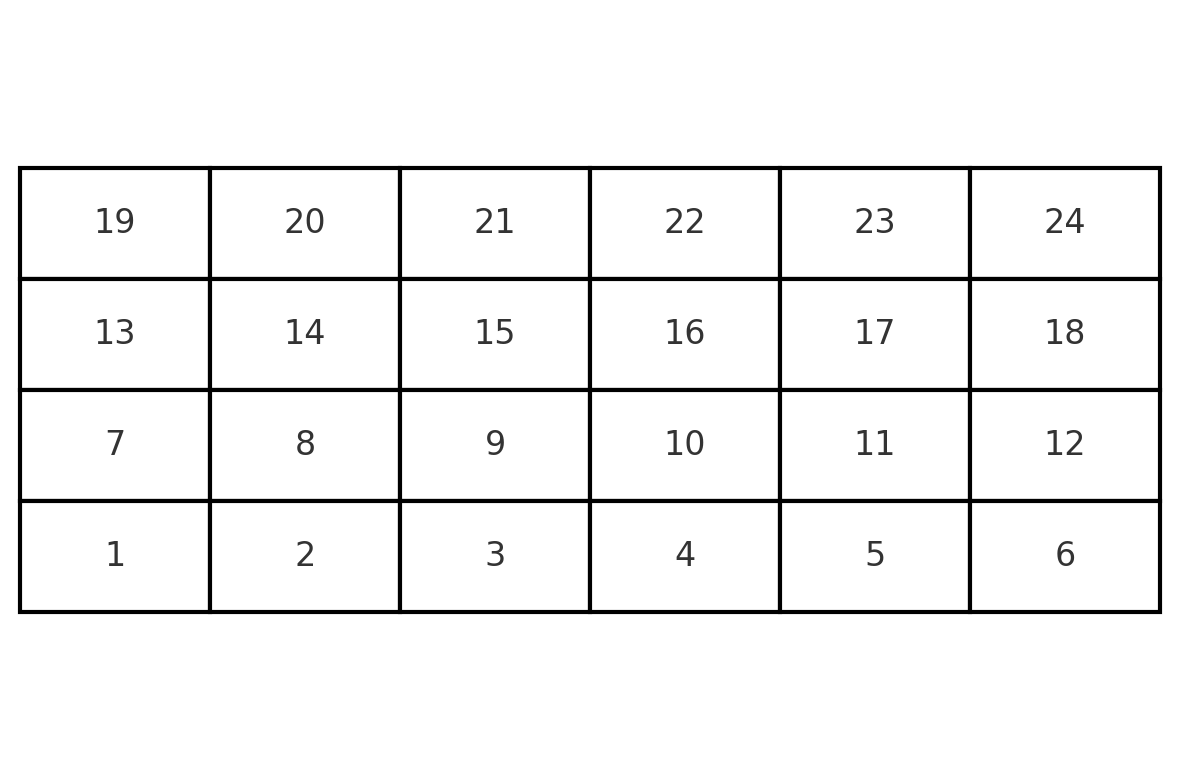
\includegraphics[width=0.6\textwidth]{plantilla-TFG-ETSIIT/doc/imagenes/Zonas_campo.png}
    \caption{Distribución en zonas del campo}
    \label{fig:etiqueta-imagen}
\end{figure}

Al igual que en los apartados anteriores, el campo se representa orientado de izquierda a derecha, de forma que las zonas 6, 12, 18 y 24 corresponden a las áreas de máximo ataque, mientras que las zonas 1, 7, 13 y 19 representan las zonas más defensivas.

Para este enfoque inicial, se han definido dos vectores de pesos: uno destinado a las estadísticas constructivas (ofensivas) y otro a las destructivas (defensivas). No obstante, en la implementación del código, ambos se gestionan como un único vector para simplificar su tratamiento.

La razón de esta separación conceptual es garantizar una evaluación adecuada del rendimiento en función del tipo de estadística. Por ejemplo, no tendría sentido asignar un peso elevado a una acción defensiva en una zona ofensiva, ya que su impacto real en el juego sería escaso. Así, el vector de ataque incrementa sus valores a medida que las zonas se aproximan al área rival, mientras que el vector de defensa lo hace en dirección contraria, aumentando su importancia conforme se acerca a la propia portería.

De este modo, se definen los siguientes vectores iniciales. A continuación, se muestra el correspondiente a las estadísticas ofensivas:

\begin{figure}[H]
    \centering
    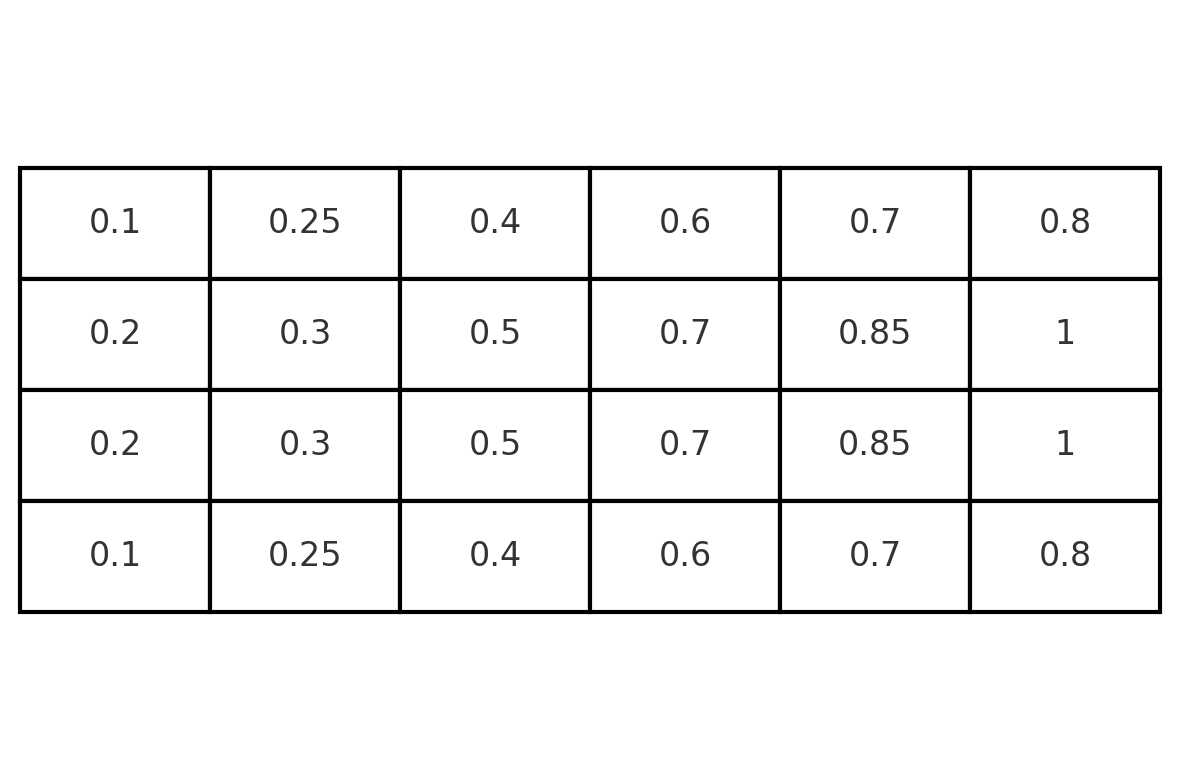
\includegraphics[width=0.8\textwidth]{plantilla-TFG-ETSIIT/doc/imagenes/Pesos_ini_ataque.png}
    \caption{Vector inicial de ataque}
    \label{fig:etiqueta-imagen}
\end{figure}

Y el vector inicial para las estadísticas defensivas:

\begin{figure}[H]
    \centering
    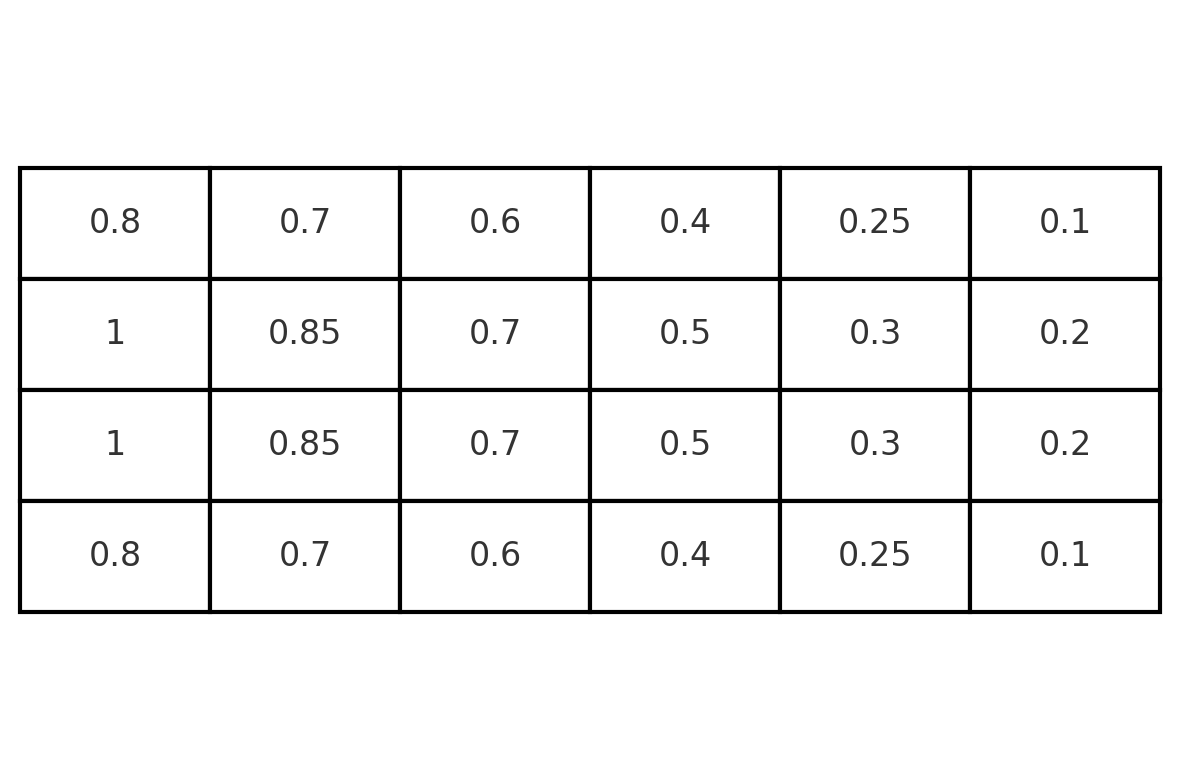
\includegraphics[width=0.8\textwidth]{plantilla-TFG-ETSIIT/doc/imagenes/Pesos_ini_defensa.png}
    \caption{Vector inicial de defensa}
    \label{fig:etiqueta-imagen}
\end{figure}

Una vez definidos los pesos correspondientes a cada zona del terreno de juego, se procede a la implementación del algoritmo. El primer paso consiste en inicializar los datos de los jugadores que han participado en el partido en cuestión. Estos datos serán la base para calcular las estadísticas ponderadas por zona, necesarias para determinar el rendimiento colectivo e individual a lo largo del campo.

\begin{lstlisting}[language=Python, caption={Inicialización datos}, label={lst:codigo-python}]
def calcula_zonas(local, visitante, temporada, corte=2):
    if not JUGADORES_CACHE:
        inicializar_cache_jugadores()

    # Obtener el partido
    partido = resultados.find_one({"Local": local, "Visitante": visitante, "Temporada": temporada})
    if not partido:
        raise ValueError(f"No se encontro el partido entre {local} y {visitante} en la temporada {temporada}.")

    jugadores1 = [jug for jug in JUGADORES_CACHE.values() if jug["equipo"] == local and jug["rival"] == visitante and jug["temporada"] == temporada]
    jugadores2 = [jug for jug in JUGADORES_CACHE.values() if jug["equipo"] == visitante and jug["rival"] == local and jug["temporada"] == temporada]
    
    preprocesar_mapa_calor(jugadores1)
    preprocesar_mapa_calor(jugadores2)

    maximos = calcularMaximos(jugadores1, jugadores2)

\end{lstlisting}

Primero se inicializan los jugadores en la caché, esto se hace para disminuir las consultas a la base de datos. De esta forma se buscan todos los jugadores una vez y se guardan en una variable llamada $\text{JUGADORES\_CACHE}$.

A continuación, se realiza una consulta para localizar el partido específico que se desea analizar, y se inicializan las variables correspondientes con los jugadores involucrados. Una vez hecho esto, se procesan los mapas de calor de cada futbolista, calculando el porcentaje de tiempo que han permanecido en cada una de las zonas del campo.

Finalmente, se determinan los valores máximos alcanzados por cada estadística entre todos los jugadores del encuentro. Estos valores se almacenan en variables locales y servirán para normalizar las estadísticas individuales, permitiendo una comparación justa y coherente entre todos los participantes.

\begin{lstlisting}[language=Python, caption={Procesamiento de cada zona}, label={lst:codigo-python}]
for z in zonas[:-1]:
        suma_total_ofensiva_e1 = 0
        suma_total_defensiva_e1 = 0
        suma_total_ofensiva_e2 = 0
        suma_total_defensiva_e2 = 0
        for j in jugadores1:
            porc = calcularPorcentaje(j, z)
            if porc != 0:
                estadisticas_ofensivas = getEstadisticasOfensivas(j["_id"], maximos) * porc
                estadisticas_defensivas = getEstadisticasDefensivas(j["_id"], maximos) * porc
                suma_total_ofensiva_e1 += estadisticas_ofensivas
                suma_total_defensiva_e1 += estadisticas_defensivas

        for j2 in jugadores2:
            porc = calcularPorcentaje(j2, z)
            if porc != 0:
                estadisticas_ofensivas = getEstadisticasOfensivas(j2["_id"], maximos) * porc
                estadisticas_defensivas = getEstadisticasDefensivas(j2["_id"], maximos) * porc
                suma_total_ofensiva_e2 += estadisticas_ofensivas
                suma_total_defensiva_e2 += estadisticas_defensivas

\end{lstlisting}

El algoritmo implementado funciona de la siguiente manera: para cada una de las zonas del terreno de juego, se recorren los jugadores de ambos equipos. Por cada jugador, se extraen sus estadísticas correspondientes, que ya han sido previamente normalizadas. Estas estadísticas se ponderan multiplicándolas por el porcentaje de influencia del jugador en la zona concreta, según lo indica su mapa de calor.

De esta forma, se obtiene una medida ajustada del impacto real de cada futbolista en cada zona del campo. Las estadísticas ponderadas se suman directamente al total correspondiente de su equipo, permitiendo así calcular una puntuación global que refleja el rendimiento colectivo en función del posicionamiento y la actividad individual de cada jugador.

\begin{lstlisting}[language=Python, caption={Procesamiento de cada zona}, label={lst:codigo-python}]
    zonas_valores_e1[z-1] = (suma_total_ofensiva_e1*zonas_coeficientes[z-1] - suma_total_defensiva_e2*zonas_coeficientes[z-1+24])
    
    zonas_valores_e2[z-1] = (suma_total_ofensiva_e2*zonas_coeficientes[z-1] - suma_total_defensiva_e1*zonas_coeficientes[z-1+24])
    
    total_rival[z-1] = (suma_total_ofensiva_e2*zonas_coeficientes[z-1] + suma_total_defensiva_e1*zonas_coeficientes[z-1+24])

suma_total = sum(zonas_valores_e1) - sum(zonas_valores_e2)

if suma_total > corte:
    return 1
elif suma_total < -corte:
    return 2
else:
    return 0

\end{lstlisting}

Una vez calculados los valores totales ofensivos y defensivos de cada equipo en cada zona del campo, el siguiente paso consiste en ponderarlos utilizando los pesos previamente definidos para cada zona. Es decir, se multiplica el valor obtenido en cada zona por su peso correspondiente, según si se trata de acciones ofensivas o defensivas.

Finalmente, se suman los resultados ponderados de todas las zonas y se comparan los totales obtenidos por ambos equipos. En función de estos valores globales, se determina el ganador del encuentro: vence el equipo con la mayor puntuación, o se declara empate si los resultados son equivalentes. Se puede ver el resultado de la ejecución de este algoritmo en el siguiente capítulo.

\section{Algoritmo genético}

Para implementar el algoritmo genético, se ha definido un único vector que representa tanto las ponderaciones ofensivas como defensivas, considerando que ambas forman parte del mismo individuo dentro de la población. Este vector tiene una longitud de 48 elementos, ya que el terreno de juego se ha dividido en 24 zonas y se asigna un peso específico a cada una, tanto para las acciones ofensivas como para las defensivas. Cada uno de los valores del vector se encuentra en el rango [0, 1], representando así la influencia relativa de cada zona en el rendimiento global del equipo.

\subsection*{Función de evaluación}
Para evaluar la calidad de un individuo, se utiliza la función evaluar\_vector, que recibe como argumento el vector de coeficientes y lo aplica a todos los partidos almacenados en la base de datos. Esta función calcula el porcentaje de aciertos que obtiene el vector al predecir los resultados. Cuanto mayor sea este porcentaje, mayor será la calidad y precisión del individuo dentro del algoritmo genético.

\subsection*{Operadores genéticos}

Para la selección se ha optado por el método de selección por torneo. Según lo expuesto por Miller y Goldberg en \cite{algoritmo_genetico}, esta técnica es muy precisa, ya que combina aleatoriedad con la elección de los mejores individuos, lo que permite mantener diversidad genética mientras se favorece la supervivencia de las soluciones más aptas.

\begin{lstlisting}[language=Python, caption={Selección por torneo}, label={lst:codigo-python}]
toolbox.register("select", tools.selTournament)
def algoritmo_genetico():
    ...
    offspring = toolbox.select(poblacion, len(poblacion) - 1,TAMANO_TORNEO)

\end{lstlisting}

El cruzamiento se realiza con una probabilidad muy alta para fomentar la diversidad entre los individuos. En las distintas ejecuciones realizadas, la tasa de cruzamiento ha sido de 0.9 o 1. Una vez seleccionados los dos vectores que se cruzarán, el proceso se lleva a cabo mediante un cruzamiento uniforme, donde cada gen tiene una probabilidad del 50\% de ser intercambiado entre ambos padres.

\begin{lstlisting}[language=Python, caption={Cruzamiento}, label={lst:codigo-python}]
toolbox.register("mate", tools.cxUniform, indpb=0.5)

def algoritmo_genetico():
        ...
        for i in range(1, len(offspring), 2):
            if np.random.rand() < TASA_CRUZAMIENTO:
                toolbox.mate(offspring[i-1], offspring[i])
\end{lstlisting}

La mutación se aplica con una probabilidad de 1 / (tamaño de población) a cada gen, es decir, a cada elemento del vector de pesos.
    
\begin{lstlisting}[language=Python, caption={Función mutación}, label={lst:codigo-python}]
def mutacion_uniforme_flotante(individuo, low=0.0, up=1.0, indpb = INDPB_MUTACION):
    for i in range(len(individuo)):
        if np.random.rand() < indpb:
            individuo[i] = np.random.uniform(low, up)
    return individuo,
\end{lstlisting}

\begin{lstlisting}[language=Python, caption={aplicación función mutación}, label={lst:codigo-python}]
toolbox.register("mutate", mutacion_uniforme_flotante, low=0.0, up=1.0, indpb=INDPB_MUTACION)

def algoritmo_genetico():
    ...
    for ind in offspring:
            toolbox.mutate(ind)
\end{lstlisting}

\subsection*{Elitismo}
Para garantizar que la mejor solución no se pierda durante el proceso evolutivo, se implementa elitismo, el cual conserva al mejor individuo de cada generación.

\begin{lstlisting}[language=Python, caption={Implementación elitismo}, label={lst:codigo-python}]
def algoritmo_genetico():
    ...
    elite = tools.selBest(poblacion, k=1)
    poblacion[:] = elite + offspring

\end{lstlisting}

\section{Algoritmo genético con $\delta$}
Con el objetivo de mejorar la precisión de la predicción, se ha decidido incluir en el vector de pesos el parámetro $\delta$, que representa el umbral de corte para decidir el resultado: si gana un equipo, el otro o si hay empate. Hasta ahora, este valor se había fijado manualmente en 2, es decir, si:

\begin{itemize}
    \item $Score global > 2$, gana local
    \item $Score global < -2$, gana visitante
    \item empate en caso contrario
\end{itemize}

El algoritmo genético, además de optimizar los vectores de ponderaciones para las zonas de ataque y defensa del campo, incluirá ahora la variable $\delta$ dentro del vector de parámetros a ajustar. La configuración del algoritmo es la misma que la descrita anteriormente, salvo por la tasa de mutación, que se ha ajustado a 1 / 49 debido al incremento en la longitud del vector. El propósito es comparar distintas técnicas para evaluar cuál ofrece un mejor equilibrio entre precisión y coste computacional.

Se probarán los mismos valores que en las ejecuciones anteriores, realizando un total de 5 repeticiones para cada combinación y calculando la media y la desviación típica de los resultados obtenidos.
